% Template LaTeX file for DAFx-08 papers % (fold)
%
% To generate the correct references using BibTeX, run
%     latex, bibtex, latex, latex
% modified...
% - from DAFx-00 to DAFx-02 by Florian Keiler, 2002-07-08
% - from DAFx-02 to DAFx-03 by Gianpaolo Evangelista
% - from DAFx-05 to DAFx-06 by Vincent Verfaille, 2006-02-05
% - from DAFx-06 to DAFx-07 by Vincent Verfaille, 2007-01-05
%                          and Sylvain Marchand, 2007-01-31
% - from DAFx-07 to DAFx-08 by Henri Penttinen, 2007-12-12
%                          and Jyri Pakarinen 2008-01-28
%
% Template with hyper-references (links) active after conversion to pdf
% (with the distiller) or if compiled with pdflatex.
%
% 20060205: added package 'hypcap' to correct hyperlinks to figures and tables
%                      use of \papertitle and \paperauthorA, etc for same title in PDF and Metadata
%
% 1) Please compile using latex or pdflatex.
% 2) If using pdflatex, you need your figures in a file format other than eps! e.g. png or jpg is working
% 3) Please use "paperftitle" and "pdfauthor" definitions below


%%%%%%%%%%%%%%%%%%%%%%%%%%%%%%%%%%%%%%%%%%%%%%%%%%%%%%%%%%%%%%%%%%%%%
%%%%%%%%%%%%%%%%%%%%%%%%%%%%%%%%%%%%%%%%%%%%%%%%%%%%%%%%%%%%%%%%%%%%%
%%%%%%%%%%%%%%%%%%%%%%%%%%%%%%%%%%%%%%%%%%%%%%%%%%%%%%%%%%%%%%%%%%%%%
% 
% TTBlue Notes / Paper
% from conversation with Dave over coffee at Pre en Bulle in Albi
% 20 June 2008
% 
% Allows for:
% * programmatic creation of user interfaces
% * adaptive wrappers for various plug-in architectures (VST, AU, Max/MSP, SuperCollider)
% * dynamic, self-modifying networks of components 
% 
% Dynamic re-configuration of the signal networks and control structures means that TTBlue can be run on a web server and the signal chain defined (or re-defined) in real time on a web client using a GUI (such as a web browser or iPhone) or SMS.
% 
% One application of this is an installation or sculptural art work where you could tweak the behavior by sending it SMS messages using a phone.



%%%%%%%%%%%%%%%%%%%%%%%%%%%%%%%%%%%%%%%%%%%%%%%%%%%%%%%%%%%%%%%%%%%%%
%%%%%%%%%%%%%%%%%%%%%%%%%%%%%%%%%%%%%%%%%%%%%%%%%%%%%%%%%%%%%%%%%%%%%
%%%%%%%%%%%%%%%%%%%%%%%%%%%%%%%%%%%%%%%%%%%%%%%%%%%%%%%%%%%%%%%%%%%%%




%------------------------------------------------------------------------------------------
%  !  !  !  !  !  !  !  !  !  !  !  ! user defined variables  !  !  !  !  !  !  !  !  !  !  !  !  !  !
% Please use these commands to define title and author of the paper:
\def\papertitle{The Jamoma Multicore Audio Graph Layer}
\def\paperauthorA{Timothy Place}
\def\paperauthorB{Trond Lossius}
\def\paperauthorC{Nils Peters}


%------------------------------------------------------------------------------------------
\documentclass[twoside,a4paper]{article}
\usepackage{dafx_08}
\usepackage{amsmath,amssymb,amsfonts,amsthm}
\usepackage{subfigure,color}
\usepackage{euscript}
\usepackage[latin1]{inputenc}
\usepackage[T1]{fontenc}    
%% %%%% for source code listing %%%%%%%%%%%
\usepackage{listings}						% required for source code listings
\lstset{language=c++}
\lstset{basicstyle=\footnotesize\ttfamily}
\lstset{commentstyle=\color{commentcolor}}
\lstset{tabsize=2}  
\lstset{gobble=2}							% eat the first tab in block listings
\lstset{aboveskip=\bigskipamount}			% amount of space above a block listing
\lstset{belowskip=\bigskipamount}			% ...
%%
\setcounter{page}{1}
\ninept

\usepackage{times}
% Saves a lot of ouptut space in PDF... after conversion with the distiller
% Delete if you cannot get PS fonts working on your system.

% pdf-tex settings: detect automatically if run by latex or pdflatex
%\newif\ifpdf
%\ifx\pdfoutput\relax
%\else
%   \ifcase\pdfoutput
%      \pdffalse
%   \else
%      \pdftrue
%\fi
%\ifpdf % compiling with pdflatex
  \usepackage[pdftex,
    pdftitle={\papertitle},
    pdfauthor={\paperauthorA, \paperauthorB, \paperauthorC, \paperauthorD},
    colorlinks=false, % links are activated as colror boxes instead of color text
    bookmarksnumbered, % use section numbers with bookmarks
    pdfstartview=XYZ % start with zoom=100% instead of full screen; especially useful if working with a big screen :-)
  ]{hyperref}
  \pdfcompresslevel=9
  \usepackage[pdftex]{graphicx}
  \usepackage[figure,table]{hypcap}
%\else % compiling with latex
%  \usepackage[dvips]{epsfig,graphicx}
%  \usepackage[dvips,
%    colorlinks=false, % no color links
%    bookmarksnumbered, % use section numbers with bookmarks
%    pdfstartview=XYZ % start with zoom=100% instead of full screen
%  ]{hyperref}
%  % hyperrefs are active in the pdf file after conversion
%  \usepackage[figure,table]{hypcap}
%\fi

\title{\papertitle}

%-------------SINGLE-AUTHOR HEADER STARTS (uncomment below if your paper has a single author)-----------------------
%\affiliation{\paperauthorA}    % This command replaces \name{The DAFx Crew}
%{\href{http://www.acoustics.hut.fi/dafx08/}{Dept. of Signal Processing and Acoustics,} \\ Helsinki University of Technology, TKK \\ Espoo, Finland\\
%{\tt \href{mailto:dafx-08@acoustics.hut.fi}{dafx-08@acoustics.hut.fi}}}
%-----------------------------------SINGLE-AUTHOR HEADER ENDS------------------------------------------------------

%---------------TWO-AUTHOR HEADER STARTS (uncomment below if your paper has two authors)-----------------------
%\twoaffiliations{\paperauthorA, \sthanks{This work was supported by the XYZ Foundation}}
%{\href{
%http://www.acoustics.hut.fi/dafx08/}{Dept. of Signal Processing and Acoustics,} \\ Helsinki University of Technology, TKK \\ Espoo, Finland\\
%{\tt \href{mailto:dafx-08@acoustics.hut.fi}{dafx-08@acoustics.hut.fi}}
%}
%{\paperauthorB,\sthanks{This guy is a very good fellow}}
%{\href{http://www.acoustics.hut.fi/dafx08/}{Reading Group, Dept.~of Reading Sciences} \\ Univ.~of Universe, Sun \\ {\tt \href{mailto:dafx-08@acoustics.hut.fi}{dafx-08@acoustics.hut.fi}}
%}
%-------------------------------------TWO-AUTHOR HEADER ENDS------------------------------------------------------

%---------------THREE-AUTHOR HEADER STARTS (uncomment below if your paper has three authors)-----------------------
\threeaffiliations{\paperauthorA, \sthanks{This work was supported by BEK, GMEA, and 74 Objects}}
{\href{http://74objects.com}{74 Objects LLC,} \\ Kansas City, Missouri, USA\\
{\tt \href{mailto:tim@74objects.com}{tim@74objects.com}}
}
{\paperauthorB,\sthanks{We are all kings here}}
{\href{http://www.acoustics.hut.fi/dafx08/}{Reading Group, Dept.~of Reading Sciences} \\ Univ.~of Universe, Sun \\ {\tt \href{mailto:dafx-08@acoustics.hut.fi}{dafx-08@acoustics.hut.fi}}
}
{\paperauthorC,\sthanks{Is still sore from ice climbing}}
{\href{http://www.acoustics.hut.fi/dafx08/}{Spinning Group, Dept.~of Turning Sciences} \\ Univ.~of Planets, Mars \\ {\tt \href{mailto:dafx-08@acoustics.hut.fi}{dafx-08@acoustics.hut.fi}}
}
%-------------------------------------THREE-AUTHOR HEADER ENDS------------------------------------------------------

%----------------FOUR-AUTHOR HEADER STARTS (uncomment below if your paper has four authors)-----------------------
%\fouraffiliations{
%\paperauthorA, \sthanks{This work was supported by BEK and GMEA}}
%{\href{http://74objects.com}{74 Objects LLC,} \\ Kansas City, Missouri, USA\\
%{\tt \href{mailto:tim@74objects.com}{tim@74objects.com}}
%}
%{\paperauthorB,\sthanks{This guy is a very good fellow}}
%{\href{http://www.acoustics.hut.fi/dafx08/}{Reading Group, Dept.~of Reading Sciences} \\ Univ.~of Universe, Sun \\ {\tt \href{mailto:dafx-08@acoustics.hut.fi}{dafx-08@acoustics.hut.fi}}
%}
%{\paperauthorC,\sthanks{She is a member of the Wheel Association}}
%{\href{http://www.acoustics.hut.fi/dafx08/}{Spinning Group, Dept.~of Turning Sciences} \\ Univ.~of Planets, Mars \\ {\tt \href{mailto:dafx-08@acoustics.hut.fi}{dafx-08@acoustics.hut.fi}}
%}
%{\paperauthorD,\sthanks{Yes, senior}}
%{\href{http://www.acoustics.hut.fi/dafx08/}{Unknown Group, Dept.~of Volatile Sciences} \\ Univ.~of Nowhere, Somewhere \\ {\tt \href{mailto:dafx-08@acoustics.hut.fi}{dafx-08@acoustics.hut.fi}}
%}
%-------------------------------------FOUR-AUTHOR HEADER ENDS------------------------------------------------------

% (end)

\begin{document}
% more pdf-tex settings:
%\ifpdf % used graphic file format for pdflatex
  \DeclareGraphicsExtensions{.png,.jpg,.pdf}
%\else  % used graphic file format for latex
%  \DeclareGraphicsExtensions{.eps}
%\fi

\maketitle


% TODO: Nils, do you know how to make the footnotes not have the annoying colored boxes around the numbers?


%%%%%%%%%%%%%%%%%%%%%%%%%%%%%%%%%%%%%%%%%%%%%%%%%%%%%%%%%%%%%%%%%%%%%%%%%%%%%%%%%%%%%%%%%%%


\begin{abstract}

Jamoma Multicore is a framework for creating graph structures in which unit generators are connected together to process multichannel audio in real-time.  The main applications currently are processing of multichannel audio signals in Max/MSP and live audio coding in Ruby.  Jamoma Multicore forms part of the Jamoma layered architecture.

% particular benefit when dealing with spatial audio

\end{abstract}


%%%%%%%%%%%%%%%%%%%%%%%%%%%%%%%%%%%%%%%%%%%%%%%%%%%%%%%%%%%%%%%%%%%%%%%%%%%%%%%%%%%%%%%%%%%


\section{Introduction} % (fold)
\label{sec:intro}

Many frameworks, toolkits, and environments for real-time audio processing fuse the issues of creating unit generators with creating graph structures that process audio through those unit generators.  Alternatively, the Jamoma Platform implements a clear separation of concerns, structured according to a layered architecture of frameworks providing a comprehensive infrastructure for creating computer music systems \cite{Place:2010}. Five frameworks currently comprise the Jamoma Platform: Jamoma Foundation, Jamoma Graphics, Jamoma Modular, Jamoma DSP, and Jamoma Multicore (see Figure~\ref{fig:layers}). Jamoma Foundation provides low-level support, base classes, and communication systems; Jamoma Graphics provides screen graphics; Jamoma Modular provides a structured approach to development and control of modules in the graphical media environment Max \cite{Place:2006} and Jamoma DSP specializes the Foundation classes to provide a framework for creating a library of unit generators. 

Jamoma Multicore is an open source C++ framework providing the ability to create and network Jamoma DSP objects into dynamic graph structures for audio processing\footnote{Licensing is provided under the terms of the GNU LGPL}.  

\begin{figure}[htbp]
\centerline{\framebox{
	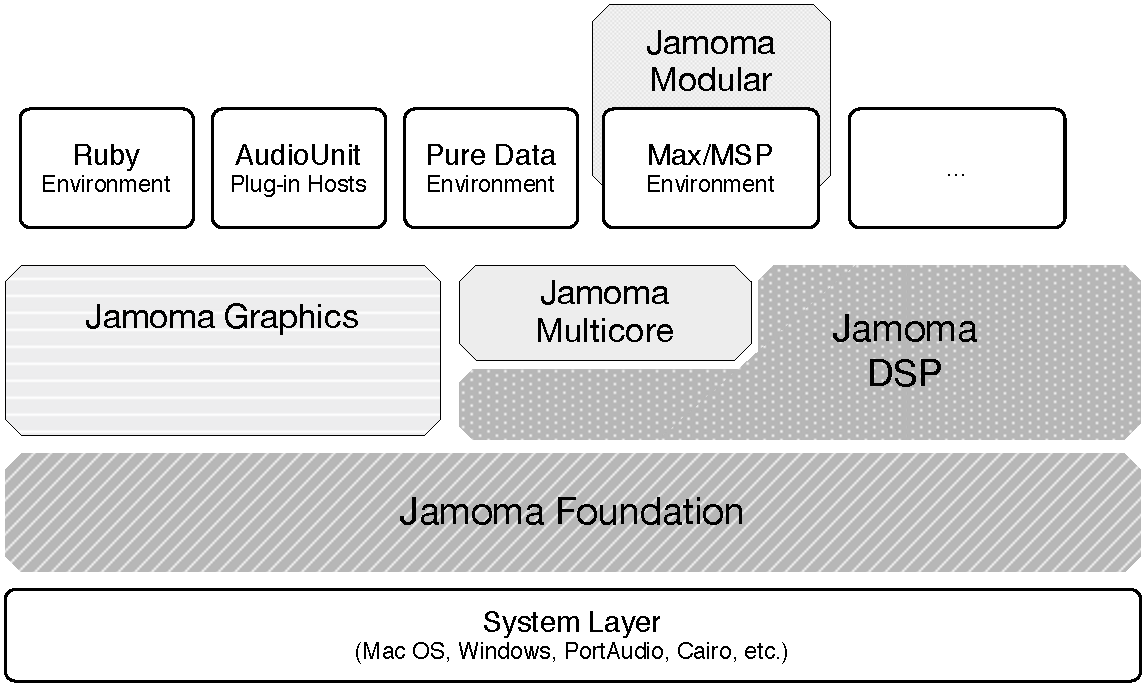
\includegraphics[width=0.9\columnwidth]{../2010-ICMC-DSP/layers-alt}}}
\caption{The Jamoma Platform as Layered Architecture.}
\label{fig:layers}
\end{figure}

In addition to the decoupling of the unit generators (Jamoma DSP) from the processing graph, Jamoma Multicore differs from other audio graph architectures in several important ways.  First, the connections between objects in the graphs are multi-channel connections; any given connection may carry N channels of audio.  Second, the content carried by the connections is dynamic; the number of channels, the size of the sample vectors, and the sample-rate of the audio can change during runtime operation.  Third, the type of graph used relies on a \emph{pull} pattern which is readily adapted to multi-threaded parallel calculations.

An additional design difference between Jamoma Multicore and most other audio processing graph software is the use of a peer object model.  The peer object model abstracts the implementation and execution of the graph from any particular environment or platform.  This allows for implementations of Jamoma Multicore to be readily implemented for any number of environments.  To date the author's have created implementations for Max, PureData, Audio Units, and Ruby.

%- presenting distinguishing between graph and units
%    - what is a graph and a unit?
%
%- requirements?
%    - be able to construct graphs
%    - multichannel as configurable 
%    - live coding (or introspection blah blah)
%  
%- additional niceties:
%    - environment-agnostic (cross-coding -  ability to prototype and wrap as plug-ins)
%
%- application for Jamoma Multicore
%    - e.g. up/downmixing; encoding/decoding 

% (end)



%%%%%%%%%%%%%%%%%%%%%%%%%%%%%%%%%%%%%%%%%%%%%%%%%%%%%%%%%%%%%%%%%%%%%%%%%%%%%%%%%%%%%%%%%%%

\section{Background} % (fold)

\subsection{Audio Graph Structures} % (fold)

A graph structure is an abstract structure where paths are created between nodes.  The paths between these nodes then define the data-flow of the graph.  Graphs targeting audio processing employ several patterns and idioms to achieve a balance of efficiency, flexibility, and real-time capability.

Virtually all audio processing graph structures are implemented using a synchronous call chain.  This simply means that the methods of the objects in the graph are called as part of a single sequence.

% in a single tick
% regularly, periodically, and atomically

synchronous vs. asynchronous

% Wikipedia:
% 
% A synchronous circuit is a digital circuit in which the parts are synchronized by a clock signal.
% In an ideal synchronous circuit, every change in the logical levels of its storage components is simultaneous. These transitions follow the level change of a special signal called the clock. Ideally, the input to each storage element has reached its final value before the next clock occurs, so the behaviour of the whole circuit can be predicted exactly. Practically, some delay is required for each logical operation, resulting in a maximum speed at which each synchronous system can run.
% To make these circuits work correctly, a great deal of care is needed in the design of the Clock Distribution Networks. Static timing analysis is often used to determine the maximum safe operating speed.
% 
% An asynchronous circuit is a circuit in which the parts are largely autonomous. They are not governed by a clock circuit or global clock signal, but instead need only wait for the signals that indicate completion of instructions and operations. These signals are specified by simple data transfer protocols. This digital logic design is contrasted with a synchronous circuit which operates according to clock timing signals.


% TODO: citation for CLAM / Amatraian

Environments for processing typically need to address concerns in both synchronous and asynchronous contexts.  For example, MIDI, setting attributes from DAW automation, etc.  These are asynchronous.  The processing of audio however, needs to be synchronous.  Most environments, such as CLAM, deal with these two types of graphs as separate from each other.  We do that too.

These synchonous calls then enforce or encourage \emph{frame processing}.  That is, processing blocks of samples at once rather than a single sample at a time.  This is also more efficient because it reduces function call overhead.

% (end)


\subsection{Push vs. Pull} % (fold)

1. What is push vs. pull

2. Examples of push : Max, Pd, ZenGarden, others? 

The Max family includes both MSP\cite{Zicarelli:1998} and PureData\cite{Puckette:1996}.

``The Max paradigm can be described as a way of combining pre-designed building blocks into configurations useful for real-time computer music performance.''\cite{Puckette:2002_max_at_17}


3. Examples of pull: AUGraph and ChucK

% Audio Units / AUGraph in CoreAudio (pull method for graphs)

``the design of ChucK strives to hide the mundane aspects of programming, and expose true control''\cite{wang:2008}.

To it's own admission, execution speed is not the primary priority for ChucK.  As such it does not perform frame-based signal computation but computes at every sample.  This contributes to ChucK's strong timing model, but at the expense of slower number-crunching for audio.

% NOTE: ChucK audio processing is driven by the sink on the graph, using a pull model as we do in Multicore 

Chuck is not multi-threaded

AUGraph does not allow ``fanning'' connections, where multiple outputs connect to single input, or a single output connects to multiple inputs.

% (end)


\subsection{Multichannel Processing} % (fold)
Discussing Max and Pd makes sense -- changing the number of channels is changing the code.

SuperCollider - mention that it is possible to work on arrays of signals in SuperCollider, while this is not easy to do in Max?

% TODO: Trond and Nils need to do a bit checking out of SuperCollider, so that we are able to do a qualified discussion of it...
% TODO: Who else has a true multichannel environment?  anyone?

% (end)


\subsection{Decoupling Graph and Unit Generator} % (fold)

We are able to create and use Jamoma DSP unit generators with a number of different graph structures.  Jamoma Multicore is one graph structure that a developer may choose to use\footnote{However unlikely, it is also theoretically possible to use Jamoma Multicore with an alternative unit generator library}.

Jamoma DSP does not define the way in which one must produce signal processing topographies.  Instead, the process of creating objects and connecting them are envisioned and implemented orthogonally and the graph is created using a separate framework known as Jamoma Multicore.  Thanks to this decoupling of Jamoma DSP and Jamoma Multicore you aren't ``boxed-in'' to any particular way of creating connections between objects.

Max, Pd, SuperCollider, Csound, Bidule, AudioMulch, Reactor, Reason all have have units, but the units can only be used within the particular environment. The units have a proprietary format for unit generators, so there's no interchangability, and likewise the graph structure is proprietary. While SDKs are available for some of them, it's not for others. For some of these no SDK exists at all, they are totally proprietary. Ability to host Audio Units and VST extends it somewhat

% (end)


\subsection{Multithreading} % (fold)

The structure of Jamoma Multicore is ideal for distributing processing of the graph amongst parallel threads.  In its current implementation it is already possible leverage multiple threads, and thus multiple processors, by running multiple graphs side-by-side in the same environment.  More powerful and dynamic opportunities arise when a graph itself is distributed to parallel threads.

%    - multithreading where applicable
%    - pragmatic multithreading: real-time statistics for optimizing between different processors
%   
%A  B
%\ /
% C



% TODO: Grand Central Dispatch (GCD) is now open source, is this relevant?

% TANGA provides and interesting environment because the audio engine is explicitly multi-threaded and thus multi-core capable\cite{Reiter:2007}.  However, it doesn't fit the bill because it is targeted at one context: MPEG-4 scene rendering.  We need something more general.  And it doesn't matter because we are thread-agnostic.

% (end)


% TODO: Is there any other environment that we should acknowledge?
% TODO: CSound?  

% (end)

%%%%%%%%%%%%%%%%%%%%%%%%%%%%%%%%%%%%%%%%%%%%%%%%%%%%%%%%%%%%%%%%%%%%%%%%%%%%%%%%%%%%%%%%%%%


\section{Design and Implementation} % (fold)

\subsection{Structure} % (fold)

Jamoma Multicore is a framework \footnote{We use the term framework in a generic sense, as a dynamically linked library together with supporting source and an API.} implementing a synchronous multichannel audio processing graph driven using a pull methodology.  This is accomplished through the creation of a node class for the graph, \emph{TTMulticoreObject}, which wraps a unit generator with other supporting objects.  \emph{TTMulticoreObject} then manages these instances and the information neccessary to pull samples from its sources.  Figure \ref{fig:anatomy} shows the classes and how they are related.

\begin{figure}[htbp]
\centerline{\framebox{
	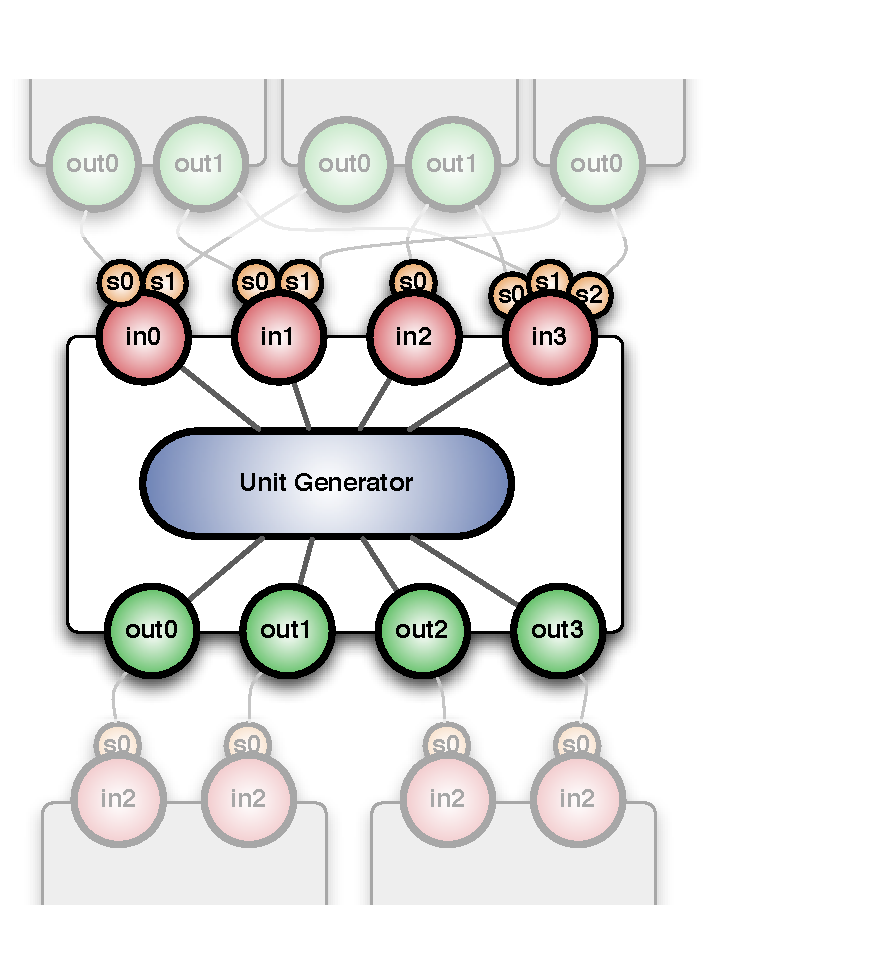
\includegraphics[width=0.9\columnwidth]{anatomy-compact}}}
\caption{MulticoreObject Class Anatomy}
\label{fig:anatomy}
\end{figure}

Since Jamoma Multicore is using a pull-based architecture, an object's \emph{outlets} are passive.  They are simply buffers storing the output calculated by the wrapped unit generator.  The unit generator is simply an instance of a Jamoma DSP class, specified as an argument when the \texttt{TTMulticoreObject} is instantiated.  This unit generator is responsible for actually calculating the audio to be stored by the outlet buffers.

Unlike the outlets, the \emph{inlets} are active.  When asked for a vector of audio by the unit generator, they then each request audio from all of their sources (other objects' outlets).  In an inlet has multiple sources, those sources are summed.  When all of the inlets have performed this operation, then the unit generator proceeds to process the audio buffered in the inlets and fills the buffers in the outlets.  Sources manage a one-to-one connection between an inlet and an outlet; inlets may have zero or more sources.  This design can be summarized thusly:

				A graph has many objects.\\
\indent	An object has many inlets.\\
\indent	An inlet has many sources.\\
\indent	A source has many channels.\\


% (end)


\subsection{Building the Graph} % (fold)

A Multicore graph consists of a collection of objects that are connected in such a way that they are able to perform digital signal processing tasks.  All processing is driven by the object at the end of the processing chain.  This \emph{terminal object} is accesses the graph by pulling from the directly-connected nodes.  Those nodes in-turn call the relevant methods on any objects connected to them, etc., until the graph access has propagated to all objects in the chain.

Before such processing can occur, the connections of the graph must be established and the graph readied for operation.  First, connections must be made.  This is done by passing a source object and an inlet number to a another object's \texttt{connect()} method.  Second, any objects connected need to be initialized by a call to their \texttt{init()} method.  This call will propagate up the tree, and so is typically only called once by the terminal object when the graph is started.  

% In our Max implementation this happens as a 3 step process:
%
% A 'reset' method is called on all Multicore objects in the graph. This tells all objects to forget any previous connections.
% 
% A 'setup' method is called on all Multicore objects in the graph. This causes objects to establish connections to other objects in the graph (i.e. by passing a message to any object directly below themselves).
% 
% An 'init' message is sent, initiated by any/all terminal Multicore objects in the graph and traversing up the graph as detailed below.

% (end)


\subsection{Processing the Graph} % (fold)

Processing the graph is a two step process.  First, a `preprocess' method is propagated up the chain from the terminal object.  This zeroes buffers and sets flags that indicate each object's processing state.  It is of no consequence if an object receives multiple preprocess calls, such as would happen if there are multiple terminal nodes.

With the objects in the graph prepared by the preprocess call, the audio can be pulled from the graph by the terminal object calling the `process' method on each of its sources.

% Third, we could send a postprocess message, but we don't at the moment.

% (end)


\subsection{Graph Description} % (fold)

Given a Jamoma Multicore graph, the topology can also be traversed for purposes other than directly calculating audio.  
Any node in a Jamoma Multicore graph can be asked for a description.  The returned \texttt{TTMulticoreDescription} object will then provide 
metadata about the entire graph as seen through that object's inlets.  
There are many applications of this description, including visual representation of the graph, statistical analysis, and cross-coding.

% (end)


% (end)



%%%%%%%%%%%%%%%%%%%%%%%%%%%%%%%%%%%%%%%%%%%%%%%%%%%%%%%%%%%%%%%%%%%%%%%%%%%%%%%%%%%%%%%%%%%

\section{Application} % (fold)

\subsection{Max/MSP} % (fold)

Show it working in Max/MSP
% TODO: need a screenshot demonstrating multi-channel

One example the demonstrates the need for dynamic vectorsizes is the gabor.psola.pat example from FTM. Also granular approaches may benefit (for example, implementing some of the ideas from Curtis Roads' engine).


\subsubsection{Jamoma Modular} % (fold)

% TODO: Tim fix jcom.unpack≈ object in subpatchers bug

Nils Says:
There is a new modular branch to start working with the multicore 
externals. The name of the branch is ``0.6-multicore''.

So far, I mainly introduced in= and out= in a couple of modules. more to come.
jmod.sur.multi.in
jmod.sur.multi.out
jmod.sur.multi.input
jmod.sur.multi.aux
jmod.sur.meters
jmod.sur.output
jmod.sur.vbap
jmod.sur.dbap

% TODO: these last two require a matrix that operates on the channels within a signal, not on multiple signals

So you can start to connect your modules and see what's working and 
what's not.
If you are curious, just check out this branch and try it.
in the git repository, go to Modules/Modular and do a

git checkout 0.6-multicore

% Some important things to keep in mind:
% - Priorities, how to we control the order of operations?    We don't at the moment (which is like Pd, but unlike Max)
% - Matrix mixer/router development, with particular thought about what happens when 5.1 audio is routed to stereo etc.
% - Signals of varying data rate (for example as proposed by Pulkki), e.g. compressed signals or higher res signals
% - Signals of steady data rate but varying vector/buffer size (as in FTM/Gabor)

Dynamic number of channels (perhaps useful for FFT and spectral processing?)

% Would be ideal if we could have a wrapper for standard MSP external objects as Multicore objects. 
% Call the DSP method directly from this wrapper?
% Create our own internal DSP chain for it?
% start simple as with biquad~, meaning 1 in and 1 out...
% it seems like the easiest way out is to just use patcher scripting.


% (end)
% (end)


\subsection{Ruby} % (fold)

Language bindings can be made for many different languages.  We have chosen Ruby.  Ruby allows lots of stuff.  

\subsubsection{Live Coding} % (fold)

One thing is Live Coding \cite{Collins:2003} using irb.  That article has some great ideas and general discussion about Live Coding.  One topic is the use of general purpose languages such as Ruby vs. domain specific languages such as ChucK.  With our extensions of the Ruby environment we hope to bridge the best of both worlds.

% TODO: Are there any published articles specifically about using irb for live coding performance?

Here is what a simple \texttt{irb} session:

\begin{lstlisting}
	require 'TTRuby'
	
 	dac = TTAudio.new "multicore.output"
 	osc = TTAudio.new "wavetable"

	dac.connect osc
	dac.send "start"
	
	osc.set "frequency", 220.0
\end{lstlisting}

% (end)

% (end)


\subsection{Cross-Coding} %(fold)

% TODO: should this go in the discussion section instead?

Code generation and prototyping...

Any node in a Jamoma Multicore graph is capable of producing a description of the graph from which it pulls audio.  This description, which is a tree structure representing the graph's topology, can then be exported to any of a number of formats.  These formats include Ruby source, C++ source, and the Max 5 JSON patcher format.

As a consequence, it is possible from any supported environment to export a representation of the graph to any other supported environment.  e.g. Max -> C++, Ruby -> Max, C++ -> Ruby, Max->Ruby, etc.

% (end)


% (end)


%%%%%%%%%%%%%%%%%%%%%%%%%%%%%%%%%%%%%%%%%%%%%%%%%%%%%%%%%%%%%%%%%%%%%%%%%%%%%%%%%%%%%%%%%%%

\section{Discussion and Future Work} % (fold)

\subsection{Multiple Simultaneous Graphs} % (fold)

By it's nature, a Multicore graph is defined as all objects connected together into a graph structure terminating at a terminal object that drives the graph.  There is no limitation on how many of these graphs may exist independently, and simultaneously, in any environment.  As these graphs are fully-independent of each other they may run at different rates, in different threads, and addressing different hardware.  The independent graphs may even run side-by-side with one running in real-time while another is operating out of real time.

% TODO: we need an object like out≈ that drives a graph outside of real time to fill a buffer~ or jit.matrix
% TODO: trond or nils -- do you have some interesting applications of the above?
% TODO: If we are presenting a graph system, should we discuss the potential (if any) for expanding this from being a graph system for audio processing, to video processing or other kinds of time-tagged data, along the line of e.g. Max/Jitter, QuartzComposer or Octane?
% TODO: Discuss the potential for work on spatialisation, and further work in this direction...
% TODO: Non-PCM streams?  The need for audio signal metadata?

A potential solution to this problem (as stated by Gino Robair):
``Because in 15 years, I will still be using my hardware synths and effects,
but I can guarantee that every bit of software I am using today, along with its sessions,
patches,
and stored settings,
will be inaccessible,
either through lack of developer support, because the host computer has died, 
or because subsequent upgrades no longer open the files I created with today's version.''

That's also the Integra problem, right?

% TODO: Also talk about the Jamoma Graph thing?


% (end)


\subsection{Multithreading} % (fold)

Multithreading is a big deal \cite{asanovic2008parallel}, \cite{multicoreICMC08}.  We can easily operate multiple graphs in their own threads as previously mentioned.  However, there are many opportunities for parallel processing within a single graph.

- Integrated Analysis and Benchmarking -- perhaps reference the upchuck operator in ChucK?
   -- This integrated analysis and benchmarking could also provide the basis by which an audio graph such as Jamoma Multicore is able to evaluate how to optimize the processes in the graph to make intelligent decisions on how to distribute the processing among threads or processors.

% (end)



\subsection{Implicit Patching} % (fold)

Marsyas is a software framework for building efficient complex audio processing systems and applications \cite{Tzanetakis:2008}. "Audio processing systems are defined hierarchically through composition using implicit patching. Both the specification of the processing network and the control of it while data is flowing through can be performed at runtime without requiring recompilation."

"It is based on a dataflow model of computa- tion in which any audio processing system is represented as a large network of interconnected basic audio process- ing units."  Just like Max/MSP, Pd, Chuck, etc.

One difference to Max/MSP and Pd is that the signal network can be reconfigured dynamically without requiring a 'recompile' of the signal chain.  This is addressed through Jamoma Multicore -- Jamoma DSP is low level and is agnostic about how objects are combined into a network or topology.

However, objects can be recombined and structured at runtime, offering the same kind of flexibility and "expressive power".

\subsubsection{Implicit Patching}

One thing that makes Marsyas special is its notion of "Implicit Patching".  In this paradigm unit generators are added to a collection and their interaction with the signal processing graph is determined according to a pattern such as 'series', 'fanout', etc. \cite{Bray:2005}.

Currently Jamoma DSP (and Multicore) operate solely through an 'explicit' patching paradigm similar to most other frameworks.  "In explicit patching the user would first create the modules and then connect them by explicit patching statements."  Due to the flexibility of the dynamically bound objects, however, it is quite easy to see how the implementation of pattern-based collections might be defined.

% (end)

% (end)

%%%%%%%%%%%%%%%%%%%%%%%%%%%%%%%%%%%%%%%%%%%%%%%%%%%%%%%%%%%%%%%%%%%%%%%%%%%%%%%%%%%%%%%%%%%
\section{Conclusions}
We rock.

% Eric Lyon had the following comment about our DSP paper, which I think could be worked-in here as a way to tie the goals of Multicore into the bigger picture:
%
%	I'm most intrigued by this statement, and would be happy to hear more about it in your paper:
%
%		"Perhaps more important, but more difficult to quantify,
%		we believe we have created a context in which code is ‚ pleas-
%		ant to work with."
%
%		This seems to be an increasingly important criterion, especially if (as I believe) we're evolving to a much more porous and flexible continuum across data-flow, scripting, and compiled coding as different entry points for musicians, depending on what they need to do. 
%
%		A few other thoughts - maybe worth writing a bit more on SuperCollider, as it is much more flexible and elegant than Max/MSP/Pd in allowing new pieces of DSP to be eased in and out of a performance (compared to the rigid poly~ structure, on the one hand, or glitches whenever new DSP objects are created on the other). 



%%%%%%%%%%%%%%%%%%%%%%%%%%%%%%%%%%%%%%%%%%%%%%%%%%%%%%%%%%%%%%%%%%%%%%%%%%%%%%%%%%%%%%%%%%%

\section{Acknowledgments}

The authors wish to thank the University of Oslo for hosting the workshop during which the initial architecture of Jamoma Multicore was designed.  We additionally thank Pascal Baltazar and everyone at GMEA for hosting a spatialization workshop during which the design of Jamoma Multicore was reviewed and heavily revised.


%%%%%%%%%%%%%%%%%%%%%%%%%%%%%%%%%%%%%%%%%%%%%%%%%%%%%%%%%%%%%%%%%%%%%%%%%%%%%%%%%%%%%%%%%%%

\bibliographystyle{IEEEbib}
\bibliography{../../Shared/bibtex/Jamoma} % requires file template.bib

\end{document}
